
%(BEGIN_QUESTION)
% Copyright 2006, Tony R. Kuphaldt, released under the Creative Commons Attribution License (v 1.0)
% This means you may do almost anything with this work of mine, so long as you give me proper credit

How much pressure, in inches of water column, is being applied to this {\it inclined} water manometer to displace water 5 inches along the length of the tube, inclined at an angle of 30$^{o}$ from horizontal?  Assume a negligible change in liquid level inside the ``well'' throughout the measurement range of the instrument:

$$\includegraphics[width=15.5cm]{i00167x01.eps}$$

\underbar{file i00167}
%(END_QUESTION)





%(BEGIN_ANSWER)

Applied pressure = 2.5 "W.C.

\vskip 10pt

What matters in manometer calculations is the {\it vertical} height difference between the two liquid columns.  Inclining one or more of the tubes only causes the liquid to displace further along the tube(s); it does not change the vertical height necessary to balance the applied pressure.

Thus, with a 30$^{o}$ inclined tube, a liquid displacement of 5 inches along the length of the tube equates to one-half that (sin 30$^{o}$ = 0.5).  Therefore, the applied pressure is 2.5 inches of water column.

Note that the inclined manometer makes very sensitive pressure measurements possible using standard-density liquids such as water!  Great care, though, must be taken in ensuring the instrument is level (that the inclined tube is at precisely the angle it should be).

%(END_ANSWER)





%(BEGIN_NOTES)


%INDEX% Measurement, pressure: inclined manometer

%(END_NOTES)


